%%%%%%%%%%%%%%%%%%%% author.tex %%%%%%%%%%%%%%%%%%%%%%%%%%%%%%%%%%%
%
% sample root file for your "contribution" to a contributed volume
%
% Use this file as a template for your own input.
%
%%%%%%%%%%%%%%%% Springer %%%%%%%%%%%%%%%%%%%%%%%%%%%%%%%%%%%%%%%%%

\title{Earthquake---Ground Shaking}
\label{chp:eq_shaking}
% Use \titlerunning{Short Title} for an abbreviated version of
% your contribution title if the original one is too long
\author{
    \textbf{Adam Zsarnóczay}
    \and Jack Baker 
    \and Wael Elhaddad
    \and David McCallen}
\tocauthor{}
\authorrunning{Zsarnóczay et al.}
% Use \authorrunning{Short Title} for an abbreviated version of
% your contribution title if the original one is too long
%\institute{Name of First Author \at Name, Address of Institute, %\email{name@email.address}
%\and Name of Second Author \at Name, Address of Institute %\email{name@email.address}}
%
% Use the package "url.sty" to avoid
% problems with special characters
% used in your e-mail or web address
%
\maketitle
\label{chapter:haz_shaking}

The simulation methods and the software tools presented in this section characterize the ground-shaking intensity due to earthquakes at a specific site or over a group of sites that cover a region. Although the amount of historical earthquake data at any particular site is small, the improvements in the field since the publication of the seminal paper on earthquake hazard by \citet{cornell1968engineering} allows engineers to combine the available information from several sites and create a seismic hazard model that can quantify the expected ground-shaking hazard and the corresponding uncertainty. 

Probabilistic Seismic Hazard Assessment (PSHA) and disaggregation of the calculated hazard are the most popular methods to characterize ground shaking at a site of interest \citep{bazzurro1999disaggregation}. The earthquake engineering community is fortunate to have access to a large number of free---and often open-source---tools available for this task. Besides PSHA tools, this chapter also covers tools that perform scenario-based, deterministic analysis. Most probabilistic and deterministic analyses use empirical ground-motion models (GMMs) that describe the attenuation of shaking intensity with increasing distance from the hypocenter to characterize the ground shaking at a site from fault rupture. [The empirical GMM denomination is preferred over the conventional GMPE (ground-motion prediction equation) in several recent publications to emphasize that modern attenuation relationships are substantially more complex than a single equation.] Other approaches, such as physics-based GMMs and the corresponding simulations, are also becoming sufficiently robust to be widely applicable for risk assessment, and they are likely to be used more widely in the near future. 

This chapter reviews the above methods, the data they use, and the tools that have implemented them. The recent book by \citet{baker2021seismic} provides more details about the characterization of ground shaking and the methods available for probabilistic seismic hazard assessment. 

\section{Input and Output Data}
\label{sec:eq_shake_io}

\subsection{Input Data}

Ground-motion hazard assessment requires information about the site and the seismic source(s) in its vicinity. These data can be classified as follows:

\paragraph{Site location(s)} These are latitude and longitude pairs for each site of interest. For regional analyses, ground shaking is either characterized directly at the location of each asset or a carefully designed intermediate grid is used, and the site-specific results are determined by interpolation between the grid nodes. The direct approach is used when the number of assets is relatively small (e.g., \cite{padgett2010regional}), while the intermediate grid is used in studies with millions of assets (e.g., \cite{deierlein2020cloud}).


\paragraph{Site data} Local soil conditions have significant influence on the ground motion at the surface at a particular site. Two neighboring sites with practically identical bedrock hazard might experience fundamentally different surface ground motions if their soil characteristics are different. If the soil profile above bedrock is available, the propagation of ground shaking from bedrock to surface can be modeled using the methods described in Chapter \ref{chapter:res_geotech} of this report. However, the bedrock is often at a large depth and the absence of site-specific measurements makes it difficult to characterize the complete soil profile. This is especially the case for large, regional simulations with thousands or millions of sites. The lack of data translates into significant uncertainty in the amplification of ground motion from bedrock to surface and the resulting surface ground-motion estimate. 

A pragmatic solution in the earthquake engineering community uses the average shear-wave velocity in the top 30 meters of the soil ($V_{S,30}$) as a proxy for soil conditions to estimate the site amplification at a site. Information about $V_{S,30}$ or at least about a broad soil class (e.g., rock, stiff soil, or soft clay) is either available or can be estimated for most sites. The USGS provides estimates of $V_{S,30}$ from topographic slope that can be used as an approximate solution when no other data is available \citep{usgs2020vs30}. 

\paragraph{Seismic sources} Ground motions are generated by seismic sources. Depending on the available historical information about the earthquakes in the region, sources might be described as faults, points, or areas with homogeneous seismicity. The abundant information about earthquakes in California allows researchers to develop a detailed map of faults for the state \citep{field2014uniform}, while the Central and Eastern United States (CEUS) is covered by area sources \citep{mueller2015seismic}.

Scenario-based analysis typically requires a hypocenter location, earthquake magnitude, and information about the rupture surface and style of faulting. Probabilistic assessments consider all sources that might affect the region along with a stochastic description of those sources using magnitude occurrence rates, hypocenter depth distributions, etc. These stochastic models are usually based on historical ground-motion data. The Uniform California Earthquake Rupture Forecast version 3.0 (UCERF3, \cite{field2014uniform}) is an example of such a stochastic seismic-source model. It is published jointly by the United States Geological Survey (USGS), the California Geological Survey (CGS), and the Southern California Earthquake Center (SCEC). Seismic-source models for other non-U.S. regions have been prepared and made publicly available by the Global Earthquake Model (GEM) initiative (\url{https://www.globalquakemodel.org/}). These include Europe \citep{giardini2014mapping}, the Middle East \citep{danciu20172014}, and South America \citep{garcia2018creation}.

\paragraph{Ground-motion model (GMM)} The ground-motion model describes the propagation of ground shaking from the earthquake rupture surface to the sites of interest. The widely used approaches are empirical, physics-based, and stochastic GMMs:
\begin{itemize}
    \item Empirical GMMs estimate the severity of ground shaking in the form of intensity measures (IMs). These estimates are typically based on regression to historical IM data from recorded earthquake ground motions. Depending on the data and the functional form used for the regression, one might arrive at various models. There are hundreds of empirical GMMs available \citep{douglas2018ground}, and it is important to select the one that is based on data and assumptions matching the seismicity in the region of interest.
    \item Physics-based GMMs describe the propagation of seismic waves from the location of the rupture to the surface at the investigated sites. They require a three-dimensional model of the local geology (i.e., the upper layers of the Earth's crust) and simulate the behavior of the seismic sources in the area within this environment. Even though these models are challenging to build and computationally expensive to run, they are becoming more and more popular, and are used in a variety of applications \citep{bradley2017guidance}. 
    \item Stochastic ground motions are artificially generated accelerograms either from white noise that is modified to match target IMs (e.g., \cite{rezaeian2011simulation}) or by modifying historical ground-motion recordings (e.g., \cite{atkinson2010inelastic, seifried2016spectral}).
\end{itemize}

\paragraph{Logic tree} Logic trees have become popular means to consider the epistemic uncertainty in the ground-shaking hazard. Branches of the trees are populated with various modeling assumptions (e.g., GMMs, seismic-source models, maximum magnitudes, site data, etc.), and a set of weights are defined so that the branches and weights represent a probability distribution on the uncertain issue. Notwithstanding the problems inherent in such a strategy for UQ \citep{bommer2008use}, recent research has shown several examples where the logic-tree approach provides additional insight that would otherwise not be available (e.g., \cite{goulet2017ngaeast}).

\subsection{Output Data}

\noindent One or more of the following outputs are produced to describe the ground-shaking hazard:

\paragraph{Seismogram} A plot of ground motion versus time, which would be recorded by a seismometer or other instrument in a real event. Seismograms are also known as ground-motion records (GMRs) and are typically expressed in terms of ground acceleration, which are integrated to obtain ground-motion velocity or displacement.  

\paragraph{Intensity measure (IM)} A measure of the intensity of shaking associated with a particular seismogram. The peak ground acceleration (PGA) and spectral acceleration at a given vibration period [\textit{Sa}(\textit{T})] are the most commonly used IMs.

\paragraph{Response spectra} A response spectrum is often used to describe the intensity of a ground motion and to provide a proxy for the complete acceleration time history. It is a collection of IMs that describe the response of single-degree-of-freedom oscillators to the ground-motion record of interest; for example, acceleration response spectra are defined through a set of \textit{Sa}(\textit{T}) values. The larger the number of vibration periods considered, the more detailed the resulting spectrum becomes. In empirical GMM-based simulations, the resolution of the response spectrum is typically limited by the vibration-period discretization used in the attenuation model. In physics-based simulations, the response spectrum is determined from the simulated GMR.

\paragraph{Hazard curve} Rather than focusing on ground motions from a single event, probabilistic assessments characterize the hazard through the annual exceedance rate of various IMs at the site of interest. This information is represented by a hazard curve. Each IM has its corresponding hazard curve. Studies typically focus on obtaining hazard curves for a set of \textit{Sa}(\textit{T}) IMs. 

\paragraph{Hazard spectrum} Given a set of hazard curves corresponding to $Sa(T_i)$ for $T_i$ in a sufficiently wide range of vibration periods, it is possible to collect the $Sa(T_i)$ that correspond to a pre-defined annual exceedance rate. These $Sa(T_i)$ values describe the so-called uniform hazard spectrum (UHS), which is the collection of spectral accelerations that have identical (uniform) probability of exceedance. A popular alternative to the UHS is the so-called Conditional Spectrum (CS), where the spectra are conditioned on the probability of exceedance of response at a pre-defined (conditioning) period $T$ \citep{lin2013conditional, baker2018improved}. The UHS and CS are often used to describe the hazard in a probabilistic framework.

\paragraph{Hazard map} Given a particular annual exceedance rate (or return period or exceedance probability over a pre-defined time period) and corresponding hazard curves at various sites in a region, one can create maps of IM levels that describe the intensity of expected ground shaking. The engineering community uses a small set of pre-defined return periods (such as 475 years, which is equivalent to 10\% probability of exceedance over 50 years) to describe the hazard for structural design and performance assessment purposes. Using the same return periods within the community facilitates the comparison of hazard maps among different regions and within different parts of the same region.

\paragraph{Disaggregation of the hazard} Probabilistic seismic hazard analysis aggregates the contributions of several sources to produce a hazard curve for a site. Disaggregation provides a break-down of the contribution of various seismic sources to the total seismic hazard. This allows researchers to estimate the characteristic features of the earthquake scenarios (typically magnitude and source-to-site distance) that are the main contributors to the seismic hazard at the site. Information about such features complements the estimated IMs and provides a more detailed understanding of the seismic hazard at the site.

\section{Modeling Approaches}
\label{sec:eq_shake_models}

The two main approaches used in the research community for ground-shaking hazard characterization are as follows:
% \newline

\paragraph{Estimate IMs using an empirical GMM} This type of methodology describes the hazard using IMs estimated based on historical earthquake data. The advantage of using empirical GMMs is the computational efficiency of the calculation; these models typically describe IMs as random variables. This approach allows engineers to estimate the probability of exceeding a pre-defined IM level given the characteristics of the earthquake scenario, the location of the site, and other parameters (soil conditions, damping, etc.). By aggregating these exceedance probabilities and the occurrence rates of corresponding earthquake scenarios over a region, engineers can arrive at the total probability of exceedance of a pre-defined IM level at the site of interest. Performing such a calculation for multiple IM levels produces the hazard curve for the site. The ground-shaking hazard is commonly described using a set of hazard curves that correspond to the spectral acceleration at various vibration periods. These hazard curves can serve as the basis of a UHS or CS for structural response estimation.

The choice of IM has been a subject of a large number of studies in recent decades (e.g., \cite{shome1998earthquakes, luco2007structure}). There are three widely-used criteria when IMs are discussed: (1) \emph{practicality} refers to the complexity of the calculation and if tools are already available to perform it; (2) \emph{efficiency} describes the predicting power of the IM for the important characteristics of structural response; and (3) \emph{sufficiency} corresponds to the uniqueness of the hazard description provided by the IM (i.e., a unique description means that GMRs with identical IM values yield identical structural responses). Besides the popular PGA and $Sa(T_1)$, the average spectral acceleration $Sa_{avg}$ and significant duration are also used and assessed in several studies (e.g., \cite{bijelic2018validation}). There are more complex IMs that have been shown to perform better in terms of efficiency and sufficiency, and can become superior to conventional choices once widely applicable GMMs become available for them (e.g., \cite{davalos2019filtered}). 

In studies that use empirical ground-motion data, the selection of historical GMRs for dynamic analyses can be challenging. One can either use a generic suite of GMRs produced and vetted by experts (e.g., \cite{baker2011new}) or perform the selection of GMRs from a database (e.g., \cite{ancheta2014ngawest2}) based on a site-specific description of the hazard. As the number of records in ground-motion databases increases, the set of selected GMRs can often provide a good representation of the probabilistic hazard at the site, but rare events and unconventional hazard characteristics can still prove difficult to represent with empirical GMRs. If matching historical ground motions are not available, stochastic ground-motion generation is also an option to consider.

\paragraph{Estimate ground-motion records using a physics-based GMM} This type of methodology relies on a physical model of the crust and propagation of seismic waves in that model. It requires a significant amount of information about local geology to arrive at reliable results. Furthermore, the calculations are computationally expensive and usually require a high performance computing (HPC) environment. To the extent that the physics-based models are validated and based on reliable model parameters (geologic data), they can represent local geologic effects (such as deep geologic basins) that are not captured as well by empirical GMMs. The earthquake simulations provide GMRs directly as opposed to the IM proxies used in empirical approaches. These records can be applied directly in response estimation, which removes part of the uncertainty and ambiguity associated with GMR selection to match IM targets in empirical studies. 

There are computational and modeling challenges before this approach becomes commonplace, but early adopters in the research community (such as SCEC  \url{https://www.scec.org/} and Lawrence Livermore National Laboratory, \url{https://www.llnl.gov}) are already providing physics-based simulations that are being applied for performance and risk assessment (e.g., \cite{frankel2018broadband, rodgers2019effect}). The SCEC Broadband Platform \citep{maechling2015scec} provides open-source access to such models and simulation tools; similar initiatives are available in Italy \citep{damico2017synthesis} and in New Zealand \citep{bradley2017guidance}. 

Concerns about the reliability of simulated ground motions have been addressed by recent studies that have shown similar demands and responses from real and simulated ground motion records (e.g., Figure \ref{fig:haz_EmpricalVsSimulated}, \cite{galasso2013validation, rodgers2019broadband}). SCEC has a group of researchers focusing on testing and rating methodologies to build confidence in the use of these simulated acceleration time histories. As the gap between empirical and simulated ground motions is closing, the community will be able to take advantage of synthetic seismograms that can represent rare hazards and special site conditions.

\begin{figure}[htb]
    \centering
    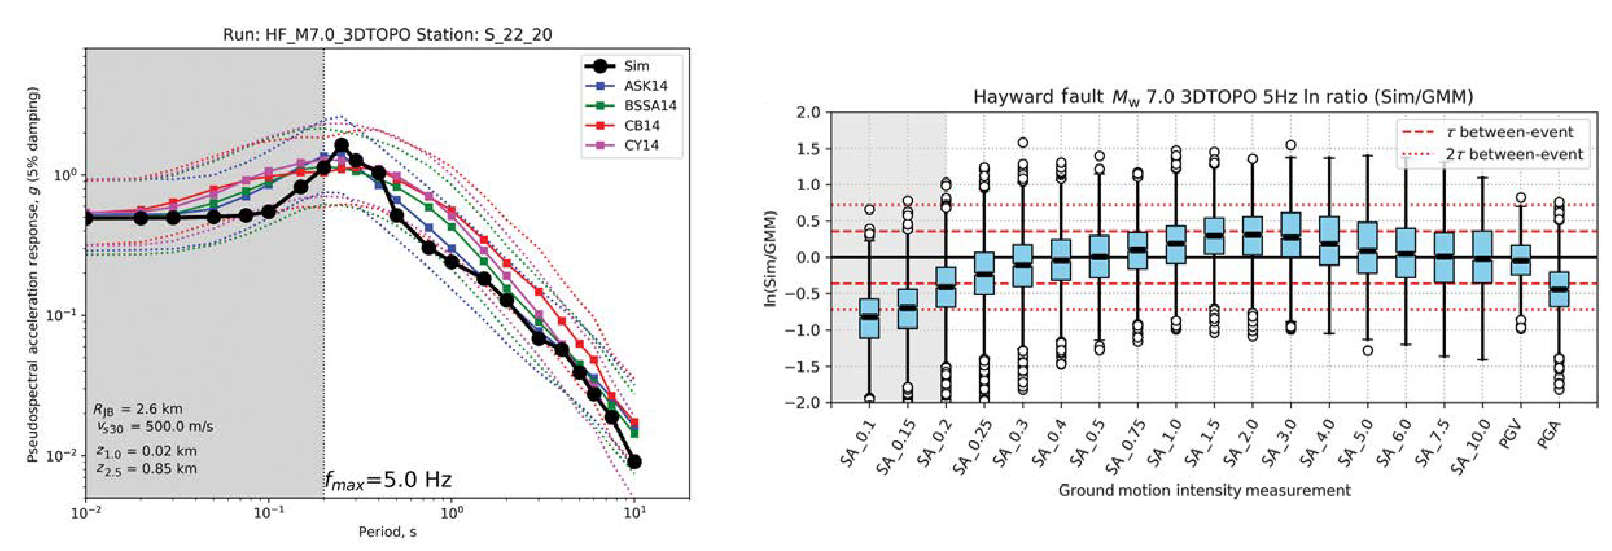
\includegraphics[width=1.0\textwidth, angle = 0]{Figures/EmpiricalVsSimulated.pdf}
    \caption{Illustrative example of the comparison between empirical and physics-based GMMs from \citep{rodgers2019broadband}: Left: RotD50 acceleration response spectra for a site in Oakland, California, predicted by four empirical GMMs (squares in color) and by a three-dimensional ground-motion simulation for the San Francisco Bay Area (circles in black). Right: Distribution of residuals between the simulated and empirical IMs over the entire simulation region. The thick black line indicates the median, the boxes show the interquartile range (IQR) (i.e., central 50\% around the median), and the whiskers extend until 1.5 IQR. Outliers are shown as circles. Dashed and dotted lines show between-event uncertainties corresponding to the empirical GMM.}
    \label{fig:haz_EmpricalVsSimulated}
\end{figure}

\section{Research Gaps and Opportunities}
\label{sec:eq_shake_gaps}

Conventional, empirical GMMs are expected to be replaced by non-ergodic models that can consider local site and path information when available (e.g., \cite{abrahamson2019probabilistic}). In areas with abundant information, such models are expected to reduce the variability in the ground motion and provide a more realistic description of the seismic hazard. Because such detailed information is not available in every location, the models need to account for site-specific aleatory and epistemic uncertainty, thus acknowledging that the uncertainty in the estimated hazard is not uniform in space. This enhanced treatment of uncertainty will also require an expansion of existing logic trees to represent the center, body, and range of the input parameters \citep{gerstenberger2020seismic}.

The rigorous combination of multiple empirical GMMs (e.g., \cite{goulet2017ngaeast}) is also a promising direction that would allow the consideration of model uncertainty in the estimated hazard. Other sources of uncertainty that affect the seismic source model---or the physical model of the crust that is used to estimate soil amplification---are also important to quantify and propagate through the analyses. 

The research community recognizes that there is long-term variability in the rate of earthquakes, and some nations have already adopted time-dependent, non-Poissonian models to have a more realistic estimate of the seismic hazard. More work is needed in this area to improve the corresponding models and to expand their use to other areas, including the hazard maps of the U.S.

When it comes to physics-based models, the continual increase in computational resources makes simulations that resolve the ground-motion time-histories up to 10 Hz and include softer soil layers in the analyses a feasible goal for the near future. As our ability to compute ground motions to ever higher frequencies increases, we are outstripping our knowledge of the subsurface geology at a fine scale. Addressing these geologic model uncertainties is one of the challenges for the community.

The next step for physics-based models would be to expand to probabilistic simulations that produce multiple plausible realizations of the ground shaking considering various sources of uncertainty in the generation and propagation of the waves. Such calculations require orders of magnitude greater computation ability than what is currently available. The challenge is to improve the physical models and frameworks to make such probabilistic analyses more feasible.

\section{Software and Systems}
\label{sec:eq_shake_tools}

The following is a list of software that is commonly used for characterizing earthquake ground shaking.

\paragraph{AWP-ODC} \citeprgm{AWP-ODC} is an elastic wave propagation program (AWP-ODC, \cite{cui2010scalable}) that performs a parallel finite-difference wave-propagation simulation. The software can simulate the dynamic rupture and wave propagation that occurs during an earthquake. It was originally written in Fortran and supports parallel computation using the message passing interface (MPI). A version of the software written in C and CUDA is also available to run on graphics processing units (GPUs).

\paragraph{BBP} The \citeprgm{Broadband} Platform \citep{maechling2015scec} is a software system developed by SCEC that can be used to generate synthetic ground motions using wave-propagation models. The BBP is distributed with data products (velocity models and Green's functions packages) that allows for the generation of seismograms for simulating historical or hypothetical earthquake scenarios in California, the northeast of the U.S., and Japan. The software runs on Linux systems and provides different seismogram generation models.

\paragraph{CyberShake} \citeprgm{CyberShake} is a computational simulation project on physics-based PSHA, developed and hosted by SCEC. CyberShake simulations have been created from studies that define the inputs, computational software, and the outputs. Outputs from studies done using CyberShake are stored in publicly accessible databases that includes studies performed for southern and central California. Data products of CyberShake include seismograms, hazard curves, disaggregation, duration results, and hazard maps.

\paragraph{HAZ} \citeprgm{HAZ} is a probabilistic seismic hazard analysis tool written and maintained by Norman Abrahamson. It is written in FORTRAN and it is not heavily documented, but it still is a popular tool for several bridge, dam, and nuclear projects.
%latest activity on the HAZ repository was in 2017 - we might not want to include it in the report

\paragraph{HAZUS 4.2} The Federal Emergency Management Agency (FEMA) has been supporting the development of \citeprgm{HAZUS4x2} for more than two decades. It is publicly available and provides a convenient way to perform regional risk assessment following the HAZUS Multi-hazard Loss Estimation Methodology 2.1 \citep{fema2011hurricanetechnical,fema2011earthquaketechnical,fema2011floodtechnical,fema2017tsunamitechnical}. The methodology covers earthquake, hurricane, tsunami, and flood hazards. Researchers and agencies in the U.S. can download input data with the tool that provides information about the hazard, the exposure (i.e., building locations and characteristics), and the vulnerability (i.e., building fragility and consequence functions) of the region. These inputs are prepared in the standard format required by the software and provide exposure data (building inventories, etc.) at a census-tract-level resolution. The software runs on Microsoft's Windows operating system and has a GUI.

\paragraph{Hercules} Hercules \citep{tu2006mesh} is a parallel finite-element wave-propagation software that can be used to simulate earthquake ruptures. It was originally developed by the Quake group at Carnegie Mellon University in collaboration with SCEC. The software is designed to be memory-efficient and highly scalable to run large-scale simulations in an HPC environment \citep{taborda2010speeding}. 

\paragraph{NSHMP-Haz} \citeprgm{NSHMP-Haz} is a Java-based library for PSHA that has been developed as part of the National Seismic Hazard Mapping Project (NSHMP) within the USGS Earthquake Hazards Program (EHP). The library is the engine driving different USGS web services and applications, which enables high-performance seismic hazard calculations required for generating hazard maps over large regions using different ground-motion models. A legacy Fortran version of this library is also available, although it is deprecated at the time of writing this report.

\paragraph{OpenSHA} \citeprgm{OpenSHA} \citep{field2003opensha} is an open-source platform for seismic hazard analysis (SHA) that was developed by the SCEC in collaboration with USGS. The platform is comprised of Java libraries and a suite of applications that are suitable for different SHA applications. For instance, OpenSHA provides graphical applications for calculating hazard spectra, hazard curves, hazard maps, hazard disaggregation, and querying site data. In addition, all the features provided by the graphical applications are available programmatically through the OpenSHA Java libraries.

\paragraph{OpenQuake Engine} \citeprgm{OpenQuake} \citep{pagani2014openquake} is an open-source library for seismic hazard and seismic risk computations. The library was developed using Python and is cross platform. The library uses data, methods, and guidelines outlined by GEM.

\paragraph{PEER Ground-Motion Database} The PEER ground-motion database (NGA-West2, \cite{ancheta2014ngawest2}) is a comprehensive set of ground-motion records from shallow crustal earthquakes in active seismic regions around the world. The database includes 21,336 records from 599 earthquake events. In addition to the ground-motion records, the database stores detailed metadata that includes different source-site distance measures, site, and rupture characterization. A web service that can perform ground-motion record selection and scaling using the records in database is also provided.

\paragraph{R-CRISIS } \citeprgm{R-CRISIS} is the latest version of the CRISIS software that has been developed by \cite{ordaz2013crisis2008} and supported by the National Autonomous University of Mexico and the Italian Department of Civil Protection. The latest version of the software is free and publicly available. It is designed to work with a GUI in a Windows environment. The software is designed to perform PSHA calculations with a large number of GMPEs built in and seismic-source models available in the literature.

\paragraph{SW4} Seismic waves, 4th order (\citeprgm{SW4}, \cite{petersson2017geodynamics}) is a software originally developed at the Lawrence Livermore National Lab (LLNL) and currently jointly developed by the LLNL and the Lawrence Berkeley National Lab under the U.S. DOE Exascale Computing Program EQSIM application framework. It can solve three-dimensional seismic wave-propagation problems. The software was developed using Fortran and C++ and makes use of a distributed memory-programming model using MPI. The software is suitable for running on HPC and is capable of producing synthetic seismograms in different formats.

\paragraph{UCVM} The Unified Community Velocity Model (UCVM, \cite{small2017scec}) is a software framework developed by SCEC that provides a common interface to query different three-dimensional seismic velocity models for the State of California. The software allows the use of alternative models to query and visualize seismic-wave velocities. The software provides query scripts to obtain the seismic-wave velocities and density visualized on a horizontal slice, cross section, and depth profile, and can also provide basin depth and $V_{s,30}$ maps. The properties provided by the velocity models included with UCVM are crucial for many wave-propagation software presented in this section.
% \newline

\paragraph{UGMS MCER} \citeprgm{UGMS-MCER} \citep{crouse2018sitespecific} is a web-based tool developed by the SCEC Committee for Utilization of Ground Motion Simulations (UGMS) to provide a site-specific maximum considered earthquake (MCE) response spectra for the Los Angeles region according to the site-specific seismic hazard analysis procedure outlined in ASCE 7-16. The tool is user-friendly and is oriented towards practitioners, and only requires the location (latitude and longitude) and site-soil classification (site class or $V_{s30}$).